
%\begin{center}
%\Large\textbf{Short-Baseline Neutrino Program}
%\end{center}

The conclusive redress of the experimental hints of sterile neutrinos thus becomes high priority for the field of neutrino physics. The Fermilab Short-Baseline Neutrino (SBN) program, shown in Fig. \ref{fig:SBNMap}, offers the unique opportunity to definitely address the ``LSND/MiniBooNE'' anomaly through the utilization of three liquid argon time projection chambers (LArTPCs) detectors and the decade old and well characterized Booster Neutrino Beam (BNB). The SBN program offers a rich physics program with the ability to perform the most sensitive search to date for the existence of sterile neutrinos at the eV mass-scale. The Short-Baseline Near Detector (SBND) will be a new 112 ton LArTPC and serve as the near detector to the SBN program located 110 meters downstream of the BNB target. SBND will measure the un-oscillated neutrino flux from the BNB and enable searches in both the neutrino appearance and disappearance channels. The MicroBooNE detector is a 89 ton active mass LArTPC located 470 meters downstream of the BNB target (just in front of the MiniBooNE experiment). MicroBooNE serves as the pioneer LArTPC experiment on the BNB and will lay the groundwork for the oscillation analysis. The far detector will utilize the upgraded ICARUS-T600 experiment, previously installed and operated at the Gran Sasso Laboratory, and will be located in a new building 600 meters from the BNB target. ICARUS's large detector mass provides the SBN program with the experimental sensitivity to definitively search for the existence of eV mass-scale sterile neutrinos.

\begin{figure}[htb]
\centering
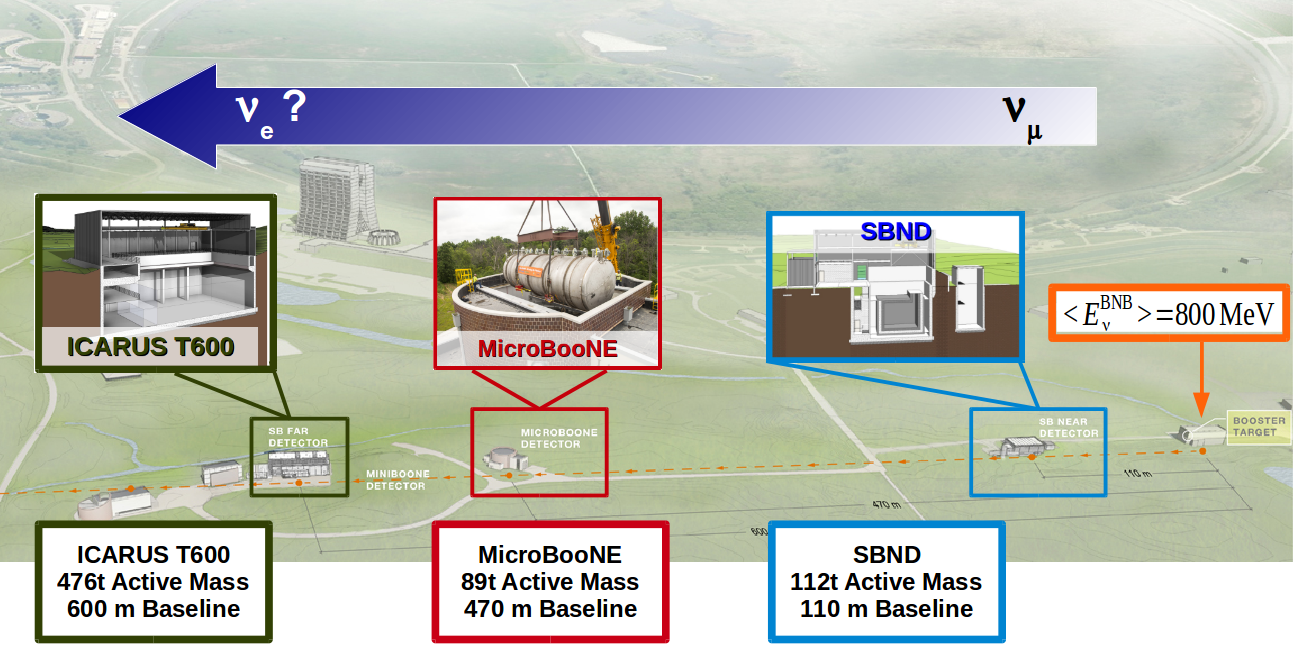
\includegraphics[width=0.65\textwidth]{images/SBNLayout2.png}
\caption[]{Overview of Fermilab's Booster Neutrino Beamline (orange dashed line) campus with the location and description of the three SBN detectors.}
\label{fig:SBNMap}
\end{figure}


The first experiment to observe an electron-like excess in the electron neutrino appearance channel was the LSND experiment \cite{No16} at Los Alamos National Laboratory. LSND used a decay-at-rest pion beam to produce muon anti-neutrinos ($\bar{\nu_{\mu}}$) in the energy range between 20-53 MeV and a distance of 30 meters from the liquid scintillator based detector. After five years of running, LSND reported an excess electron like events corresponding to a 3.8$\sigma$ evidence for $\bar{\nu_{\mu}} \rightarrow \bar{\nu_{e}}$ oscillations occurring with a $\Delta m^{2}$ of $\sim 1$eV$^{2}$. This suggests an oscillation beyond the SM three flavor neutrino oscillation which occurs at an $L/E_{\nu} \sim 1$m/MeV. To test for the appearance of this anomalous oscillation, the MiniBooNE experiment \cite{No17} at Fermilab utilized 700 MeV muon neutrinos produced from the Booster Neutrino Beam at a baseline of 540 meters (thus giving a similar $L/E_{\nu}$ to LSND). MiniBooNE identified muon and electron neutrino interactions by their characteristic Cherenkov rings inside a scintillator detector. As shown in Figure \ref{fig:minibooneExcess}, in ten years of data taking in both neutrino and anti-neutrino running MiniBooNE observed a 3.5$\sigma$ excess in $\nu_{e}$ candidates and a 2.8$\sigma$ excess in $\bar{\nu_{e}}$ candidates. This excess of events observed by MiniBooNE can be due to electrons from $\nu_{e}$ interactions as well as from single photon backgrounds, since these two final states are indistinguishable to the Cherenkov imaging detector.

\begin{figure}[htb]
\centering
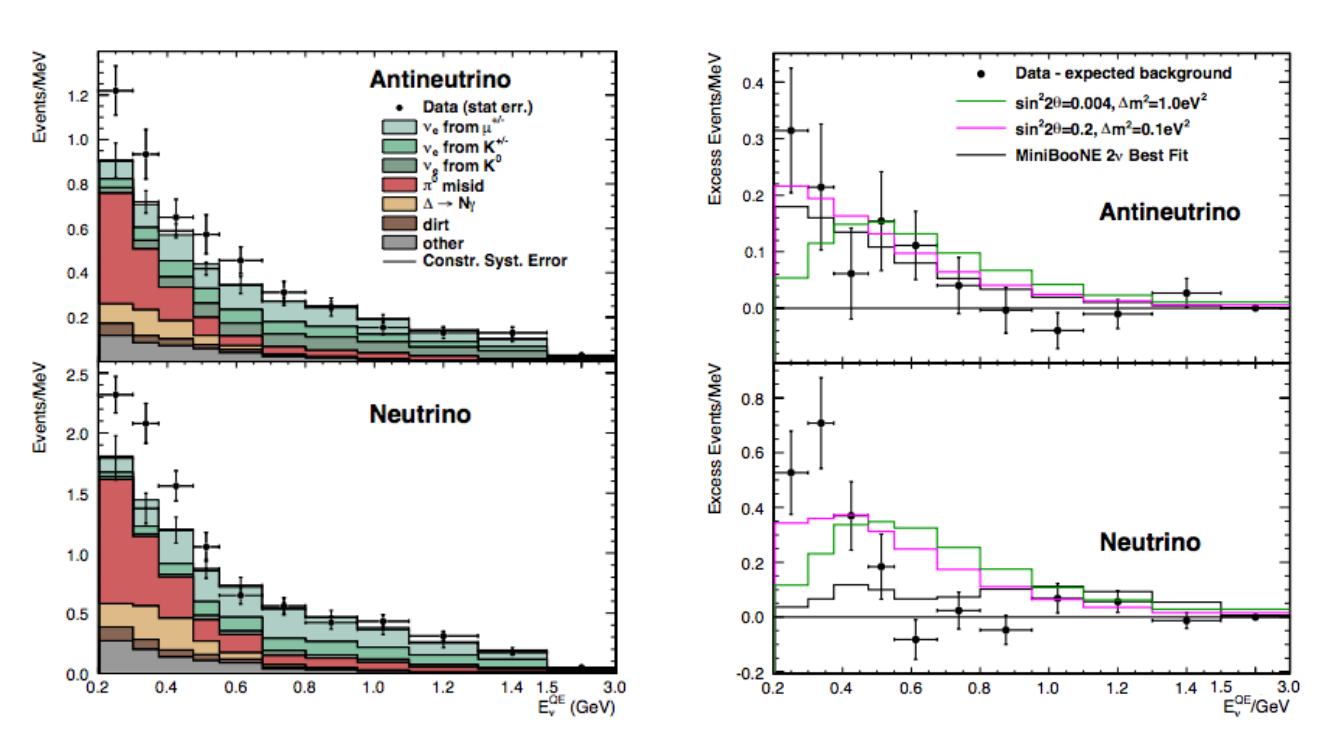
\includegraphics[width=0.85\textwidth]{images/minibooneExcess.png}
\caption[]{Left: Electron anti-neutrino ($\bar{\nu_{e}}$) and neutrino ($\nu_{e}$) candidate events shown with the predicted backgrounds in MiniBooNE. Right: Background subtracted event rates in MiniBooNE as well as different sterile neutrino models overlayed with the data.}
\label{fig:minibooneExcess}
\end{figure}

A common interpretation of this data is to posit the existence of one or more additional sterile neutrino states with masses at or below the eV range. This interpretation requires mixing of the sterile state(s) with both the electron and muon neutrino flavor states. Constraints from sterile mixing from $\nu_{\mu}$ and neutral current disappearance data \cite{No18, No19} leads to significant tension between the $\nu_{e}$ appearance data and the $\nu_{\mu}$ disappearance data. 

To disentangle the open question of how to interpret the LSND/MiniBooNE anomaly, both an excellent neutrino detector technology as well as a robust experimental program is required.  The liquid argon time projection chamber (LArTPC) offers physics capabilities ideally suited for the study of neutrino interactions. By combining millimetre scale tracking capabilities, outstanding calorimetry by having a fully active/sampling detector, and powerful particle identification made by combining the ionization along the particle trajectory (dE/dX) and the topological information, LArTPCs have been chosen to be the premier neutrino detector technology. 

